% Compilation commands
% lualatex paper.tex
% makeglossaries paper
% bibtex paper
% lualatex paper.tex

\documentclass[a4paper,10pt,twocolumn]{article}

% Page margins and layout
\usepackage[margin=2cm]{geometry}
\usepackage{multicol}
\setlength{\columnsep}{0.7cm}

% glossary
\usepackage[acronym, toc]{glossaries}
\makeglossaries
\usepackage[backend=bibtex, style=numeric]{biblatex}
\addbibresource{references.bib}

% Font and encoding
% \usepackage[utf8]{inputenc} % only pdflatex
% \usepackage[T1]{fontenc} % only pdflatex
\usepackage{lmodern}

% Math
\usepackage{amsmath, amssymb, bm}

% Graphics and plots
\usepackage{graphicx}
\usepackage{caption}
\usepackage{subcaption}
\usepackage{float}
\usepackage{pgfplots}
\pgfplotsset{compat=1.18}

% Tables
\usepackage{booktabs}
\usepackage{multirow}
\usepackage{array}
\usepackage{tabularx}
\usepackage{caption}

% Lists
\usepackage{enumitem}
\setlist{nosep}

% Hyperlinks
\usepackage[hidelinks]{hyperref}

% Glossary entries
\newglossaryentry{shift-invariant}{
    name=shift-invariant,
    description={Un kernel \`e shift-invariant se e solo se la sua trasformata di Fourier non cambia con la traslazione del contenuto dell'immagine}
}
\newglossaryentry{blind-deconvolution}{
    name=blind-deconvolution,
    description={Metodo di estrazione di ground-truth image in cui il blur kernel \`e ignoto}
}
\newglossaryentry{non-blind-deconvolution}{
    name=non-blind-deconvolution,
    description={Metodo di estrazione di ground-truth image in cui il blur kernel \`e noto}
}

% Title and author
\title{\textbf{Rete Convoluzionale per Image Deblurring}}
\author{Gruppo}
% \date{\today}

\begin{document}

\twocolumn[
\maketitle
\begin{abstract}
    L'obiettivo del progetto \`e l'applicazione di una U-Net Convoluzionale al fine di migliorare la qualit\`a dell'immagine in input rimuovendo il Blur causato dal moto del soggetto acquisito
    (\textit{Motion Blur}) o causato dalla messa a fuoco dell'obiettivo (\textit{Focus Blur})
\end{abstract}
\vspace{1em}
]

\section{Introduction}\cite{convir}

\section{Theory and Traditional Approach}

Una immagine con Blur \`e modellata matematicamente come convoluzione tra ground-truth image latente e blur kernel, dove si quest'ultimo essere \textit{\gls{shift-invariant}}. In questo caso,
l'estrazione dell'immagine sharp \`e un problema di \textit{Image Deconvolution}, la quale \`e suddivisa in \textit{\Gls{non-blind-deconvolution}} e \textit{\Gls{blind-deconvolution}}.\par
Formulazione Matematica:

\begin{math}
    \bm{b} = \bm{i} * \bm{k} + \bm{n}
\end{math}

Dove:

\begin{itemize}[topsep=0pt, noitemsep]
    \item[] $\bm{b}$: Immagine con blur
    \item[] $\bm{i}$: Immagine \textit{ground-truth} latente
    \item[] $\bm{k}$: Blur Kernel
    \item[] $\bm{n}$: Rumore presente nell'immagine per contare imperfezioni causate dall'acquisizione (quantizzazione, saturazione del colore, risposta non linare della camera, ...) (Esempio: rumore gaussiano)
\end{itemize}

\paragraph*{Non-Blind Deconvolution}

In questa metodologia tradizionale, il blur kernel \`e noto a priori (Esempio: Point Spread Function Gaussiana per Blur senza direzione, Linea con direzione e lunghezza per Blur con direzione).\par
Uno dei primi metodi utilizzati in questa categoria, implementato come comparazione, \`e la \textit{Wiener Deconvolution}, il cui obiettivo \`e la ricerca di un filtro $\bm{g}$ tale che, tramite
convoluzione con l'immagine blurred $\bm{b}$. Espresso nel dominio di Fourier:

\begin{align}
    \hat{\bm{I}} &= \bm{G}\bm{B} \\
    \bm{G}       &= \frac{|\bm{K}|^2}{|\bm{K}|^2+\frac{1}{\mathrm{SNR}}} \frac{1}{\bm{K}}
\end{align}

Dove:

\begin{itemize}[topsep=0pt, noitemsep]
    \item[] $\bm{G}$ e $\bm{K}$: trasformate di Fourier di $\bm{g}$ e $\bm{k}$
    \item[] $\mathrm{SNR}$: Signal to noise ratio (infinitamente alto se rumore assente)
\end{itemize}

Un'implementazione di tale metodo di Deblurring si basa su un metodo di ottimizzazione convessa chiamato \textit{Alternating Direction Method of Multipliers} (ADMM)\footnote{\url{https://stanford.edu/class/ee367/reading/lecture6_notes.pdf}}

\paragraph*{Blind Deconvolution}

In questa metodologia, il blur kernel \`e ignoto\footnote{I metodi con neural network rientrano in questa categoria}, dunque parte dell'algoritmo \`e la \textit{PSF estimation}, modellata come
stima di una stima di densit\`a di probabilit\`a

\section{Architettura del modello}
L'architettura utilizzata corrisponde in buona parte a quella illustrata in~\cite{convir}. La rete si basa su di una struttura a U (encoder-decoder convoluzionali), con estrazione delle feature effettuata a risoluzioni multiple (downsampled)
e con l'aggiunta dei cosiddetti \textit{Multi-Scale Modules} (\textit{MSM}), che hanno l'obiettivo di implementare meccanismi di attenzione di diversa forma (quadrata e rettangolare).

\begin{figure*}[t]
\centering
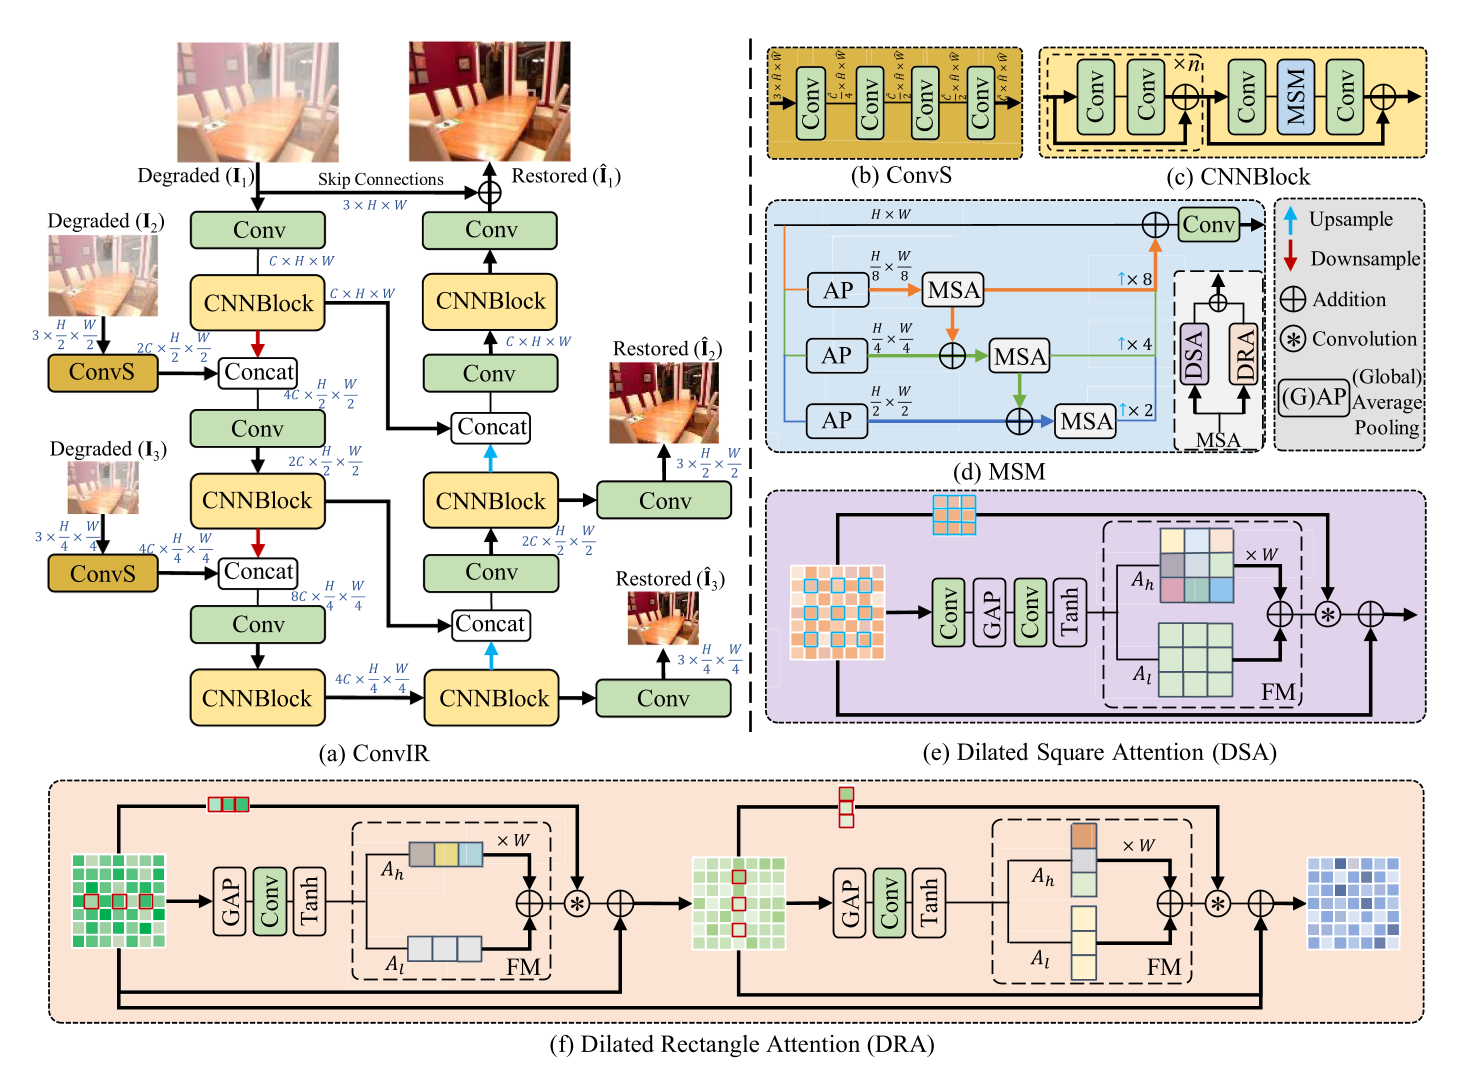
\includegraphics[width=\linewidth]{figures/architecture_complete.png}
\caption{Schema generale dell'architettura completa (ConvIR)}
\label{fig:architecture}
\end{figure*}

In figura~\ref{fig:architecture} è riportata l'architettura completa. La prima caratteristica interessante è che l'immagine in input viene elaborata non solo alla risoluzione primaria (256x256) generata dal dataloader,
ma viene ulteriormente sottocampionata (rispettivamente alla metà e a un quarto della risoluzione) e reinserita nella rete come input dei layer successivi.
L'obiettivo di questa configurazione multi-input multi-output è di analizzare l'immagine degradata secondo diversi livelli di dettaglio, e quindi di individuare pattern e feature più variegati e di diversa intensità.

L'encoder e il decoder hanno una struttura pressoché speculare, con tre skip connection che collegano i due rami, corrispondenti alle tre differenti risoluzioni a cui viene elaborata l'immagine. Come avviene di consueto nelle reti convolutive,
al ridursi della dimensione del tensore in larghezza e altezza, cresce il numero di canali. La feature extraction passa infatti attraverso i seguenti moduli:
\begin{enumerate}[label=\textbf{(\alph*)}]
    \item layer convolutivo semplice (blocco \textit{Conv} in verde in figura);
    \item \textit{ConvS}, blocco utilizzato solo per le versioni sottocampionate dell'immagine in input: consiste in una sequenza di quattro layer convolutivi che mantengono costanti le dimensioni di larghezza e altezza;
    \item \textit{CNNBlock}, blocco costituito da una serie di layer convolutivi raggruppati in \textit{n+1} blocchi residuali; nell'ultimo di questi blocchi viene inserito anche il \textit{MSM};
    \item \textit{MSM} (\textit{Multi-Scale Module}): fonde l'elaborazione di tre moduli \textit{MSA} (\textit{Multi-Scale Attention}), che operano appunto su tre scale dimensionali gradualmente decrescenti.
            Ogni \textit{MSA} combina di fatto l'output di un \textit{DSA} e un \textit{DRA};
    \item \textit{DSA} (\textit{Dilated Square Attention}): produce prima una attention map concentrandosi sulle aree quadrate del tensore in input, attraverso layer convolutivi e di pooling,
            e in seguito la elabora attraverso un filtro passa alto con parametri allenabili che sottrae unicamente la componente continua e tende ad esaltare quelle a più alta frequenza, 
            tipicamente responsabili del blur;
    \item \textit{DRA} (\textit{Dilated Rectangle Attention}): modulo analogo al precedente ma focalizzato su pattern di forma rettangolare, combina attention map in senso verticale e orizzontale.
\end{enumerate}
La loss function utilizzata corrisponde alla somma pesata di un contributo calcolato nel dominio spaziale (\(\mathcal{L}_1\)) e uno in frequenza (\(\mathcal{L}_{freq}\)), in modo da considerare adeguatamente i diversi apporti dovuti alla presenza del blur:
\[
\mathcal{L}_1 = \mathcal{L}_{spatial} = \sum_{i=1}^{3}\frac{1}{P_i} \left\lVert \hat{\mathbf{I}}_i - \mathbf{Y}_i \right\rVert _1,
\]
\[
\mathcal{L}_{freq} = \sum_{i=1}^{3}\frac{1}{S_i} \left\lVert [\mathcal{R}(\hat{\mathbf{I}}_i), \mathcal{I}(\hat{\mathbf{I}}_i)] - [\mathcal{R}(\mathbf{Y}_i), \mathcal{I}(\mathbf{Y}_i)] \right\rVert _1,
\]
dove \(i\) indicizza gli output multipli a diverse risoluzioni; \(\hat{\mathbf{I}}\) e \(\mathbf{Y}\) rappresentano rispettivamente l'immagine elaborata dalla rete e il ground truth;
\(P\) e \(S\) indicano il numero totale di elementi dei tensori presi in considerazione, in modo da avere delle metriche normalizzate;
gli operatori \(\mathcal{R}()\) e \(\mathcal{I}()\) estraggono rispettivamente la parte reale e immaginaria della FFT operata sull'immagine.\\
La funzione di costo complessiva è così calcolata:
\[
\mathcal{L}_{tot} = \mathcal{L}_{spatial} + \lambda\mathcal{L}_{freq},
\]
dove \(\lambda\) è un iperparametro impostato di default a \(0.01\). 

\section{Observations}

\section{Results}

\printglossary[title=Glossary, toctitle=Glossary]

\printbibliography

\end{document}
